\let\negmedspace\undefined
\let\negthickspace\undefined
\documentclass[journal]{IEEEtran}
\usepackage[a5paper, margin=10mm, onecolumn]{geometry}
%\usepackage{lmodern} % Ensure lmodern is loaded for pdflatex
\usepackage{tfrupee} % Include tfrupee package

\setlength{\headheight}{1cm} % Set the height of the header box
\setlength{\headsep}{0mm}  % Set the distance between the header box and the top of the text

\usepackage{gvv-book}
\usepackage{gvv}
\usepackage{cite}
\usepackage{amsmath,amssymb,amsfonts,amsthm}
\usepackage{algorithmic}
\usepackage{graphicx}
\usepackage{textcomp}
\usepackage{xcolor}
\usepackage{txfonts}
\usepackage{listings}
\usepackage{enumitem}
\usepackage{mathtools}
\usepackage{gensymb}
\usepackage{comment}
\usepackage[breaklinks=true]{hyperref}
\usepackage{tkz-euclide} 
\usepackage{listings}
% \usepackage{gvv}                                        
\def\inputGnumericTable{}                                 
\usepackage[latin1]{inputenc}                                
\usepackage{color}                                            
\usepackage{array}                                            
\usepackage{longtable}                                       
\usepackage{calc}                                             
\usepackage{multirow}                                         
\usepackage{hhline}                                           
\usepackage{ifthen}                                           
\usepackage{lscape}
\begin{document}

\bibliographystyle{IEEEtran}
\vspace{3cm}

\title{6.5.9}
\author{EE24BTECH11015 - Dhawal}

% \maketitle
% \newpage
% \bigskip
{\let\newpage\relax\maketitle}

\renewcommand{\thefigure}{\theenumi}
\renewcommand{\thetable}{\theenumi}
\setlength{\intextsep}{10pt} % Space between text and floats

\textbf{Question:}

Find the maximum value of the function $f\brak{x}=\sin x +\cos x$
\\

\textbf{Theoretical Solution}\\
For maxima $f^\prime\brak{x}=0$ and $f^{\prime\prime}\brak{x} \leq 0$
\begin{align}
    f^\prime\brak{x} &= \cos x -\sin x =0\\
    sinx&=cosx
\end{align}
We get $x=\frac{\pi}{4}$ and $x=\frac{5\pi}{4}$\\
Lets check $f^{\prime\prime}\brak{x} \leq 0$\\
\begin{align}
    f^{\prime\prime}\brak{x} &= -\sin x -\cos x 
\end{align}
For $x=\frac{\pi}{4}$\\
\begin{align}
    f^{\prime\prime}\brak{x} &= -\sqrt{2} \leq 0
\end{align}
We get,
\begin{align}
    x_{max} = \frac{\pi}{4}=0.785392&,\quad y_{max} =\sqrt{2}= 1.414214
\end{align}

\textbf{Computational Solution}
\begin{align}
    f^\prime\brak{x_{n}} &= \cos x_n -\sin x_n
\end{align}

Gradient ascent to find local maximum,
\begin{align}
    x_{n+1} &= x_{n} + \eta f^\prime\brak{x_{n}} \\
	x_{n+1} &= x_{n} + \eta \brak{\cos{\brak{x_{n}}}-\sin{\brak{x_n}}}
\end{align}

Where $\eta$ is the learning rate.

Assuming,
\begin{align}
    \eta &= 0.1 \\
    \text{tolerance} &= 1e-6 \\
    x_{0} &= 0.0
\end{align}

We get,
\begin{align}
    x_{max} = 0.785392&,\quad y_{max} = 1.414214
\end{align}

\begin{figure}[h]
    \centering
    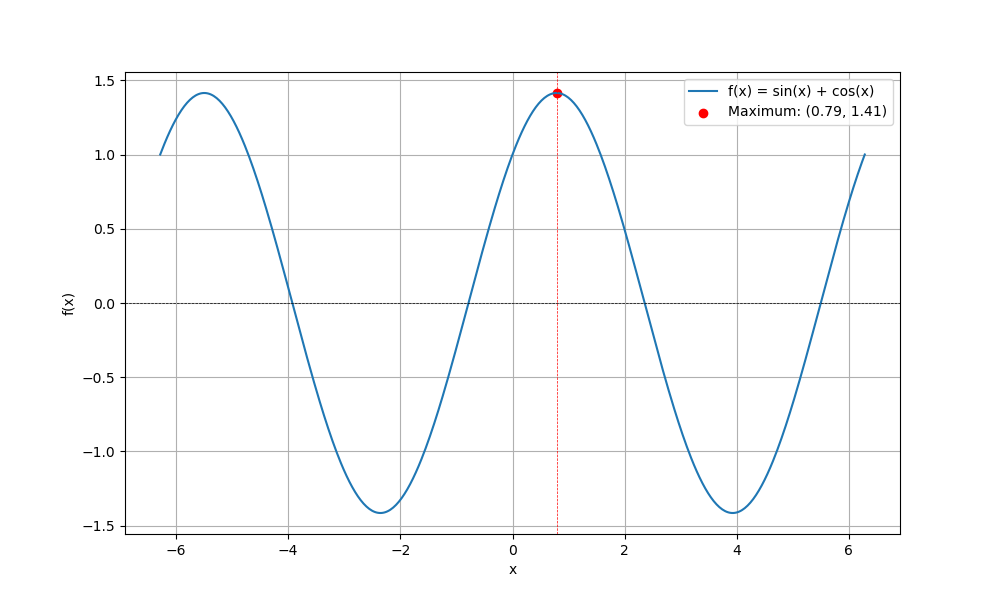
\includegraphics[width=\columnwidth]{figs/Figure_1.png}
    \label{fig:Plot}
    \end{figure}


\end{document}
